\clearpage
\makeatletter
\efloat@restorefloats
\makeatother


\begin{appendix}
\hypertarget{comparing-bayesian-and-frequentist-models}{%
\section{Comparing Bayesian and Frequentist
models}\label{comparing-bayesian-and-frequentist-models}}

Bayesian and Frequentist models have fundamentally different theoretical
interpretations and therefore, implications for the interpretation of
the coefficients provided by the statistical model. We will illustrate
the differences between Bayesian and Frequentist model estimates in a
linear mixed effects models analysis of the copy-task components. The
model is fitted on the log-transformed inter-keystroke intervals with
copy-task component as fixed effects and random intercepts for
participants and bigrams. To evaluate the fit of this model, we fitted
an intercept-only model without the fixed effect for copy-task
component.

The linear mixed effects model fitted in lme4 showed a statistically
significant fit (\(F\)(5)=4,047.55, \(p\) \textless{} .001; AIC =
47,297.49). The model with copy-task component as fixed effect rendered
a better fit compared to the intercept-only model and was found more
informative (\(\chi^2_5\) = 552.80, \(\Delta\)AIC = 544.80).

The Bayesian linear mixed effects model with copy-task component as
fixed effect rendered a predictive performance of
\(\widehat{elpd}\)=-231,643.79 (\(SE\)=297.70). The predictive
performance was found to be better compared to the intercept-only model
(\(\Delta\widehat{elpd}\)=-249.80, \(SE\)=25.02). This model comparisons
provides inference akin to the Frequentist linear mixed effects model.

The coefficients for each copy-task component estimated by the
Frequentist and Bayesian linear mixed effects model are shown in Figure
\ref{fig:lmms}. Estimates were determined by the Frequentist and
Bayesian linear mixed effects model ({[}B{]}LMM). The estimate of
Bayesian model is the maximum a posteriori, the most probable parameter
estimate. The lower and upper bound are the 95\% confidence intervals
for the Frequentist model and the 95\% highest posterior density
interval (HPDI) for the Bayesian model. The parameter estimates and the
associated intervals show a general difference between the Tapping task,
the HF bigram component, and the Sentence task one the one hand, and the
LF bigram component and the Consonant copying task on the other hand.

\begin{figure}[!h]

{\centering 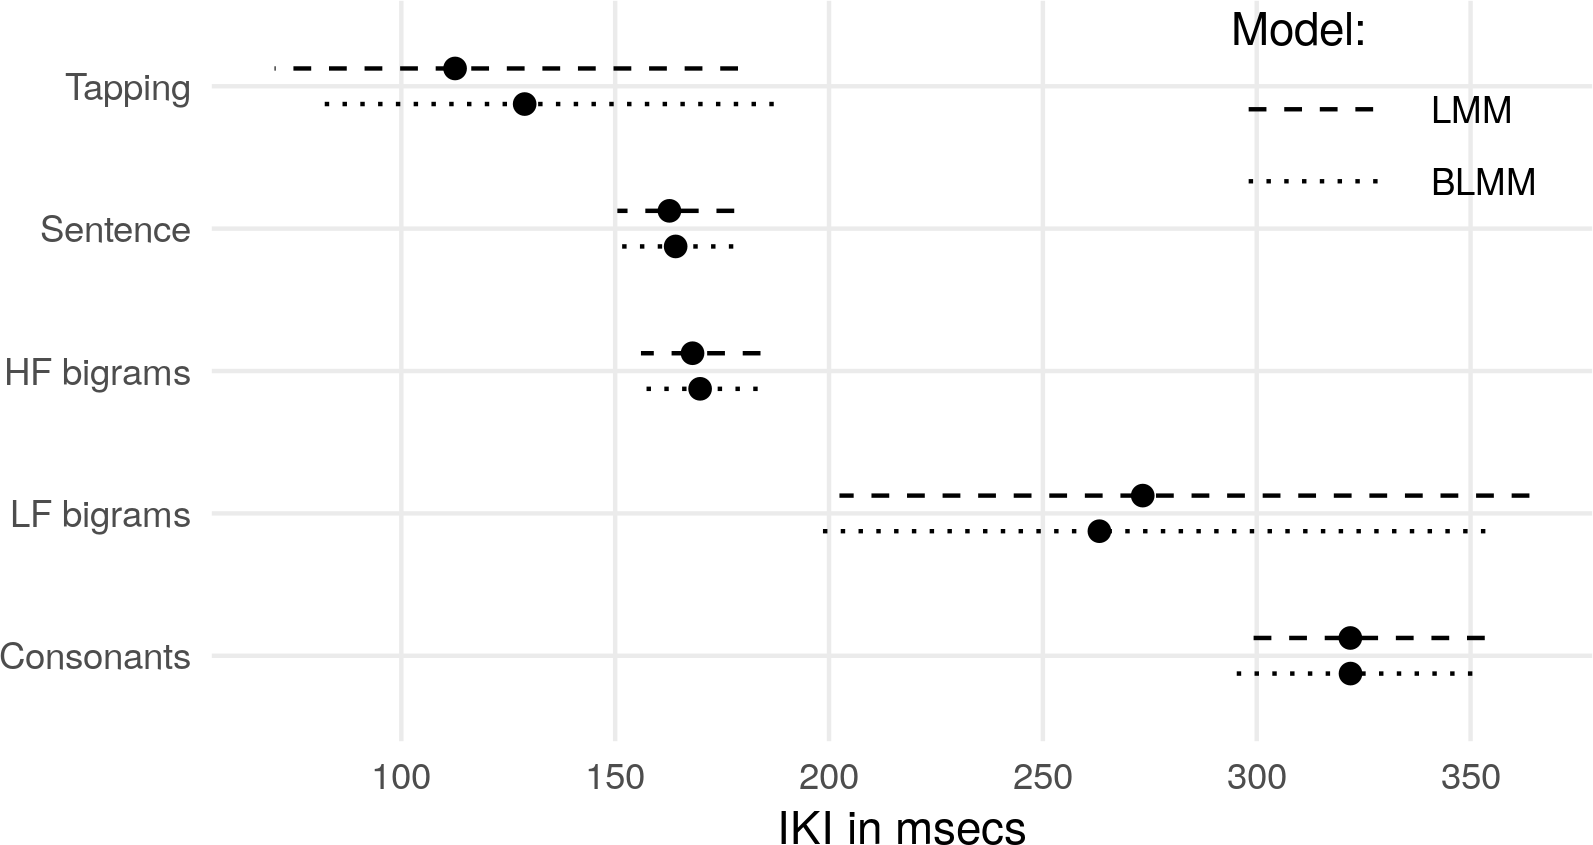
\includegraphics{ct_files/figure-latex/fig0-1} 

}

\caption{\label{fig:lmms}Model estimates of the inter-keystroke intervals (IKI) for each copy-task component estimated in a Bayesian and Frequentist linear mixed effects model ([B]LMM). Dots show the parameter estimate and intervals show 95\% CIs for the LMM and 95\% HPDIs for the BLMM.}(\#fig:fig0)
\end{figure}

Overall, the coefficients are numerically very similar, if not
identical. However, the interpretation is crucially different. The
estimate of Bayesian model is the \textit{maximum a posteriori}. This
coefficient represents the most probable parameter estimate of the
unknown true effect. The Frequentist estimate has no such probability
associated to it. Akin for the lower and upper interval bounds. The
lower and upper bound for the Frequentist model are the 95\% confidence
intervals (CI). For the Bayesian model, the interval shows the 95\%
Highest Posterior Density Interval (HPDI). Although the intervals look
very similar the interpretation is not the same at all. The HPDI is
defined as the shortest interval containing 95\% of the posterior
probability mass and represents the area in which the largest amount of
posterior estimates lie. Bayesian HPDIs, probability/percentile
intervals and credible intervals all provide the probability range in
which the true parameter value lies with the highest certainty. 95\% CIs
have a more involved definition and can be understood to represent the
amount of intervals that would contain the true parameter value if we
were to repeat an experiment a large number, if not infinite, number of
times under the same conditions. Therefore, 95\% CIs cannot be
understood as an intervals that contains a true parameter value with a
probability of 95\%, whereas Bayesian posterior intervals do have this
interpretation.

As Bayesian models provide probability distributions of parameter
estimates, we can derive inference directly from the model's posterior.
The distributions of the parameter estimates as shown in Figure
\ref{fig:blmm}. From these distributions we can calculate the
probability of observing keystroke-intervals below or above a particular
threshold or within a particular range. For example, from the posterior
shown in Figure \ref{fig:blmm} we can determine that in the Tapping task
the probability of observing keystroke intervals below 100 msecs is
0.16, below 80 msecs is 0.02 and below 50 msecs is 0. For the Consonants
component, the probability of observing keystroke intervals for all of
these thresholds is 0. In contrast, the probability to observe keystroke
intervals above 350 msecs is 0.03 for the Consonants components but 0 in
the Tapping task.

\begin{figure}[!h]

{\centering 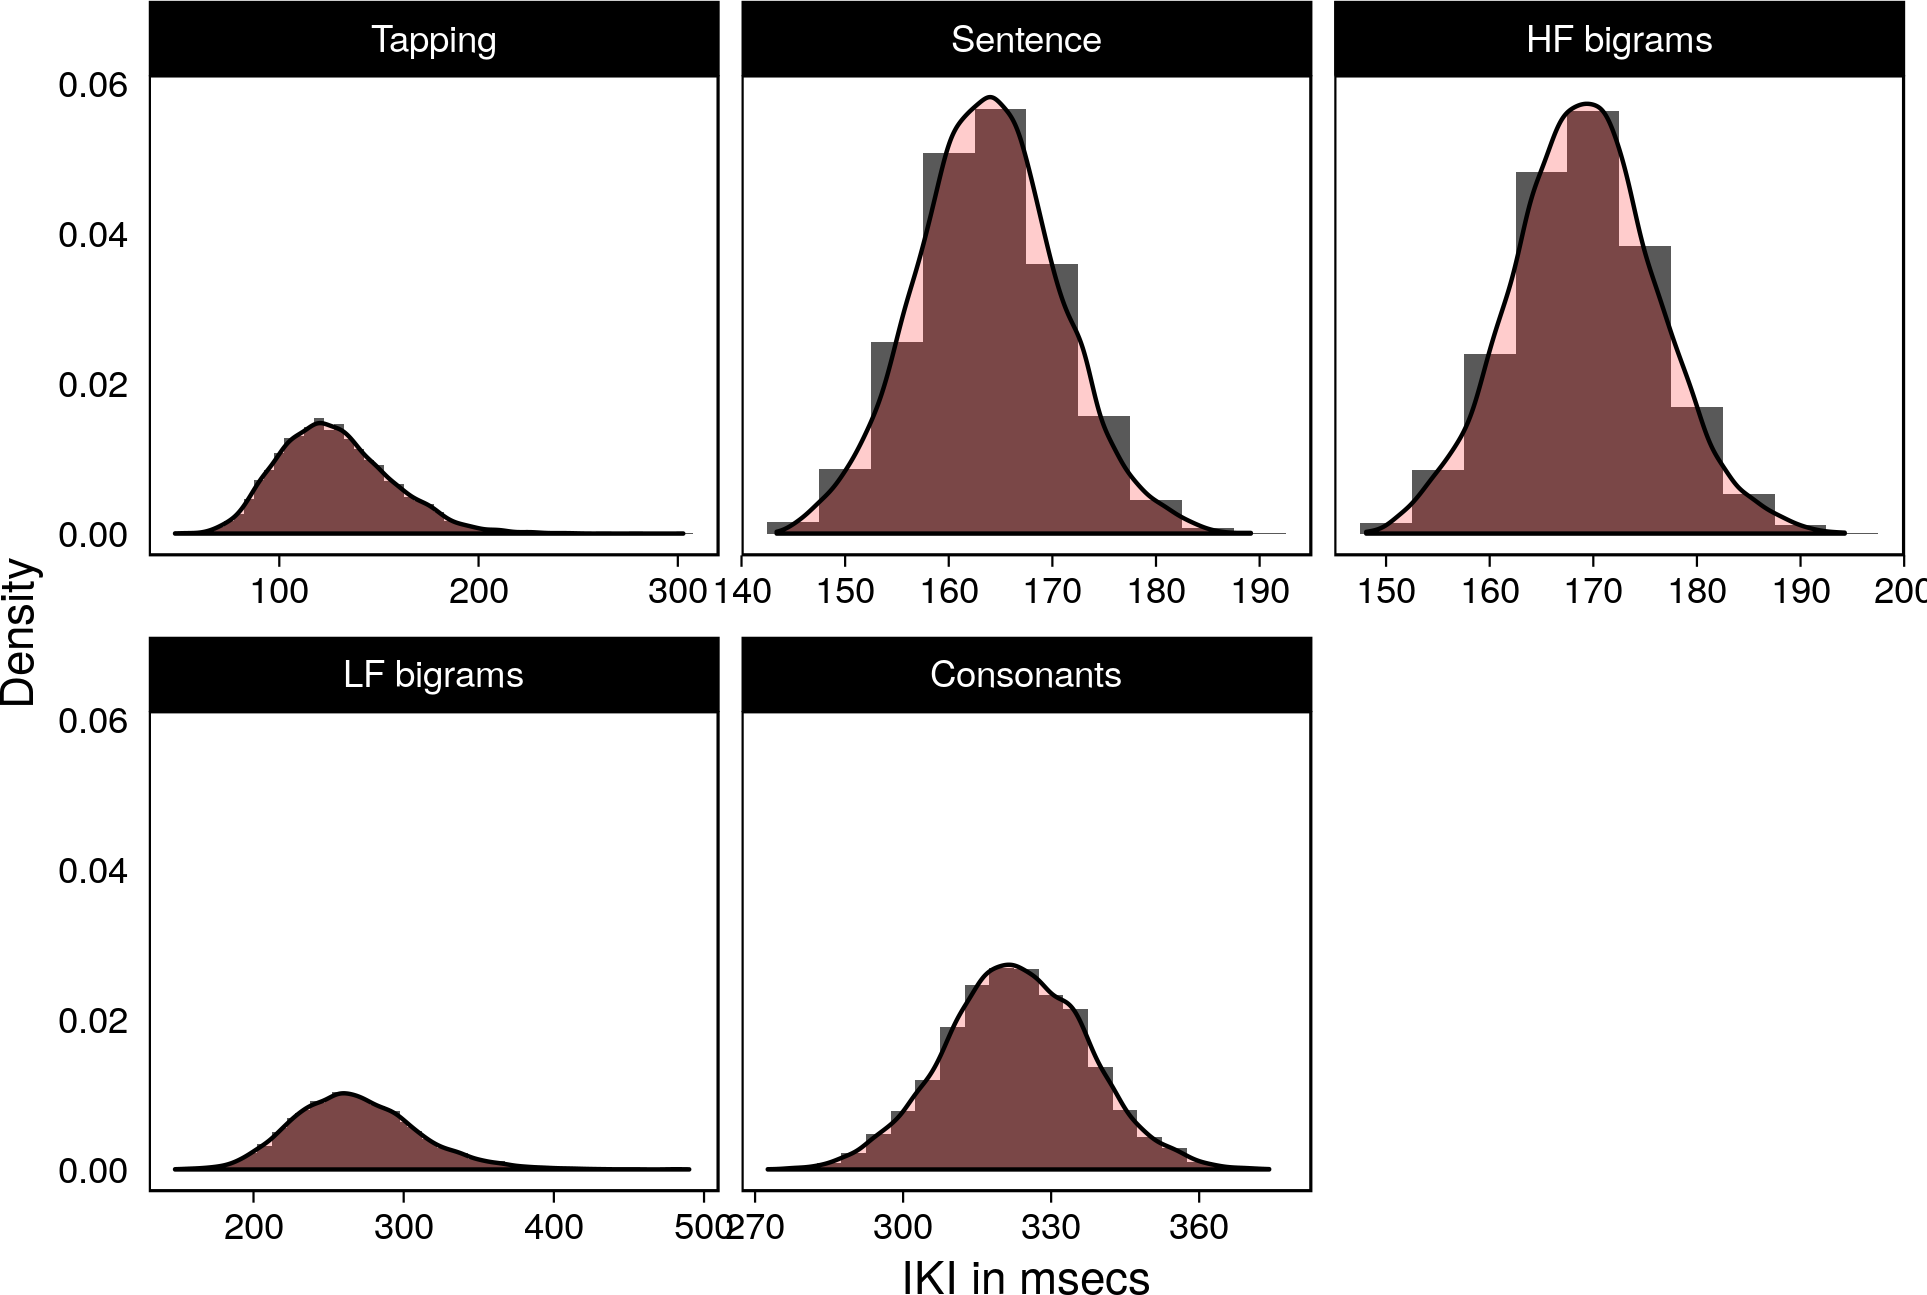
\includegraphics{ct_files/figure-latex/fig1-1} 

}

\caption{\label{fig:blmm}Histograms of the posterior probability distribution of inter-keystroke intervals (IKI) generated from the BLMM.}(\#fig:fig1)
\end{figure}

The interpretive difference between Bayesian and Frequentist statistics
rests on the property that statistical inference in Bayesian statistics
uses (posterior) probability distributions. In other words, the derived
model estimates are associated with a probability distribution.
Frequentist quantities do not have this property and reply on assumed
replications. Bayesian models, in contrast, allow us to test our
hypotheses directly using the data at hand.

\hypertarget{data-trimming}{%
\section{Data trimming}\label{data-trimming}}

Extremely deviating interkey intervals that are often considered as
noise were not removed for the following reasons. A bottom threshold
defined at 30 msecs which has been argued to indicate unintentional
double strokes or continuous key pressing does not apply as non-targeted
bigrams were removed. As can be seen in the left panel of Figure
\ref{fig:outliers} any other threshold on the lower end would need to be
arbitrary and is difficult to be justified by the data. As for an upper
threshold, following Hoaglin \& Iglewicz (1987), we may consider 1827
msecs.\footnote{Hoaglin \& Iglewicz (1987) defined outliers based on the
  differences between quartile 3 (Q3) and quartile 1 (Q1) means. This
  interval is multiplied by factor 2.2. The upper threshold for outliers
  is then calculated by adding this score to Q3. We applied this formula
  to the slowest component, i.e.~the consonant task. This resulted in
  the following calculation: ((Q3 \(-\) Q1) \(\times\) 2.2) \(+\) Q3
  \(=\) ((772.93 \(-\) 293.59) \(\times\) 2.2) + 772.93 \(=\) 1,827.47 }

The right panel of Figure \ref{fig:outliers} illustrates the
distribution of data above the determined threshold. This proposal,
however, hinges on the assumtion that the data follow a normal
distribution which we know is not the case in human response time data.
Data are positively skewed which results from the fact that response
time data are zero bound (Baayen, 2008). In other words, inter-keystroke
intervals can be infinitely slow but not faster than or equal to 0
msecs. More generally, trimming on the upper end would affect in
particular the data of participants that are slow typists (e.g.~many
elderly participants) and those copy-task components that are more
challenging (e.g.~the consonant task) but extreme values in faster
components, such as the tapping task, or in usually fast typists would
be disregarded. Therefore, instead of removing values that might be
considered extreme, we used statistical methods that are able capable of
accounting for large values.

\begin{figure}[!h]

{\centering 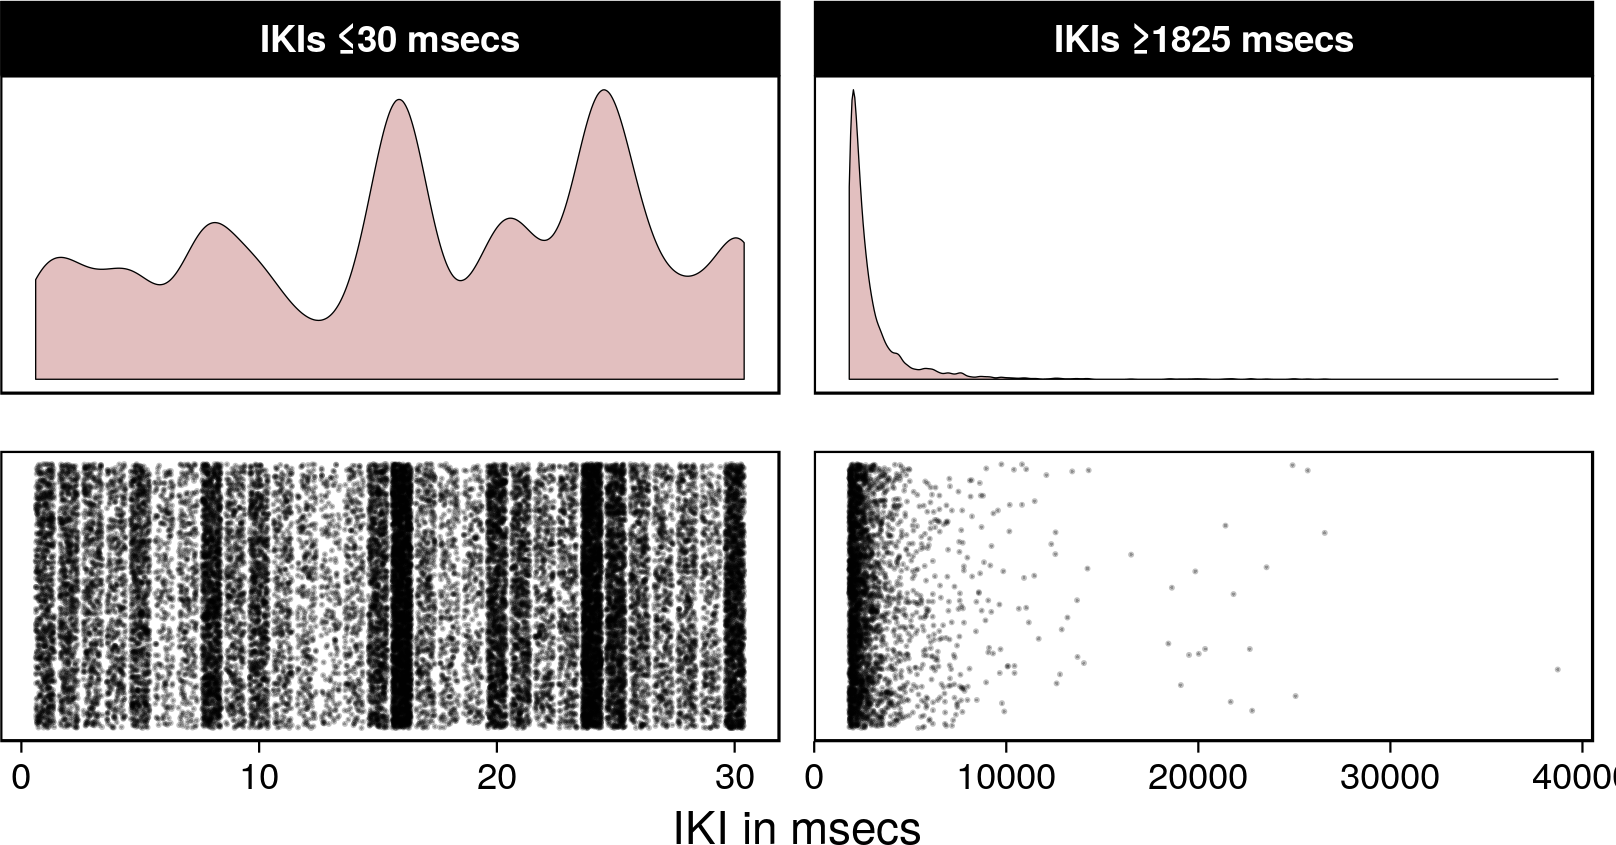
\includegraphics{ct_files/figure-latex/fig0a-1} 

}

\caption{\label{fig:outliers}Distribution of inter-keystroke intervals shown on the lower (left panel) and upper (right panel) extreme. Graphs show the density distribution of the data in the top panel and the jittered individual data points on the lower panel.}(\#fig:fig0a)
\end{figure}

\hypertarget{refs}{}
\leavevmode\hypertarget{ref-baa08book}{}%
Baayen, R. H. (2008). \emph{Analyzing linguistic data. A practical
introduction to statistics using R}. Cambridge: Cambridge University
Press.

\leavevmode\hypertarget{ref-hoaglin1987fine}{}%
Hoaglin, D. C., \& Iglewicz, B. (1987). Fine-tuning some resistant rules
for outlier labeling. \emph{Journal of the American Statistical
Association}, \emph{82}(400), 1147--1149.
\end{appendix}
